\documentclass{article}
\usepackage[utf8]{inputenc}
\usepackage{graphicx}
\usepackage{amsmath }
\usepackage{amssymb}
\usepackage{subcaption}
\usepackage{float}
\usepackage{mathtools}
\setcounter{section}{1}


\usepackage{cleveref} %referencing figures, equations and tables
\crefformat{figure}{Figure.~#2#1#3}
\crefformat{equation}{Eq.~#2#1#3}
\crefformat{table}{Table.~#2#1#3}
\crefformat{appendix}{Appendix.~#2#1#3}
\crefformat{section}{Section.~#2#1#3}

\title{The Impact Analysis of Two Identical Bars Using The Wave Equation and d'Alembert Solution}
\author{Amir Baharvand }
\date{}

\begin{document}

\maketitle

The d'Alembert solution to wave equation in one-dimension, \cref{eq:dalembert_sol}, includes two main terms: (a) $f(x + ct)$ which indicates a backward wave moving in the negative direction of $x$-axis (see \cref{fig:p2} for the direction of $x$-axis) and (b) $f(x - ct)$ that is a forward wave moving in the positive direction of $x$-axis. 

\begin{equation}
    u(x, t) = \frac{1}{2} [f(x + ct) + f(x - ct)]
    \label{eq:dalembert_sol}
\end{equation}

Invoking the chain role and assuming linear elasticity, the velocity, $v$, and longitudinal stress, $\sigma$, can be calculated from the following equations.

\begin{align}
    & v(x, t) = \frac{\partial u(x, t)}{\partial t} = c f'(x + ct) - c f'(x - ct) \notag\\ 
    & \sigma(x, t) = E \epsilon = E \frac{\partial u(x, t)}{\partial x} = E [f'(x + ct) - f'(x - ct)]
    \label{eq:v_s}
\end{align}

in which $E$ is the Young's modulus and $\epsilon$ is longitudinal strain. \\

In the case of impact of two identical bars with similar $\rho$, $A$ and $l$, to avoid misinterpretation as well as input conflict in Maple, we may use the following forms of wave equation where the second backward wave is replaced with letter $g$ and subscripts 1 and 2 denotes bars $s1$ and $s2$, respectively.

\begin{align}
    & u_1(x, t) = \frac{1}{2} [g_1(x + ct) + f_1(x - ct)] \notag\\ 
    & u_2(x, t) = \frac{1}{2} [g_2(x + ct) + f_2(x - ct)]
    \label{eq:dalembert_sol12}
\end{align}

Consequently, $v$ and $\sigma$ become

\begin{align}
    & v_1(x, t) = c g_1'(x + ct) - c f_1'(x - ct) \notag\\
    & \sigma_1(x, t) = E [g_1'(x + ct) - f_1'(x - ct)] \notag\\
    & v_2(x, t) = c g_2'(x + ct) - c f_2'(x - ct) \notag\\
    & \sigma_2(x, t) = E [g_2'(x + ct) - f_2'(x - ct)]
    \label{eq:v_s12}
\end{align}

The set of equations in \cref{eq:v_s12} along with suitable initial and boundary conditions can be used in analyzing the impact of bars. \\

Suppose the problem in \cref{fig:p2} where the bar $s1$ hits the stationary bar $s2$. The problem can be broken into different time intervals.

\section{$t = 0$}
At $t = 0$, both bars are stress-free and the bar $s1$ has the initial velocity $v_0$. As $s1$ hits $s2$, a compressive wave is generated at the contact area and propagates towards the left and right in $s1$ and $s2$, respectively which are essentially $g_1$ and $f_2$ terms in \cref{eq:dalembert_sol12}. At this time the following initial and boundary conditions can be written.

\begin{align}
    & v_1(x, 0) = v_0 \Rightarrow c g_1'(x) - c f_1'(x) = v_0 \notag\\
    & \sigma_1(x, 0) = 0 \Rightarrow E [g_1'(x) - f_1'(x)] = 0 \notag\\
    & v_2(x, 0) = 0 \Rightarrow c g_2'(x) - c f_2'(x) = 0 \notag\\
    & \sigma_2(x, 0) = 0 \Rightarrow E [g_2'(x) - f_2'(x)] = 0
    \label{eq:t0}
\end{align}

Using \texttt{dsolve} command from Maple gives 

\begin{align}
    & g_1(x) = \frac{v_0 x}{2c} + c_2 \notag\\
    & f_1(x) = -\frac{v_0 x}{2c} + c_4 \notag\\
    & g_2(x) = c_1 \notag\\
    & f_2(x) = c_3
    \label{eq:t0_ans}
\end{align}

$c_1$ to $c_4$ are constants and are not required to be determined as they vanish in calculating velocity and longitudinal stress. \cref{eq:t0_ans} shows that at $t = 0$, $s1$ is characterized by the two backward ($g_1(x + ct)$) and forward ($f_1(x - ct)$) waves. Substituting \cref{eq:t0_ans} in \cref{eq:t0} gives

\begin{align}
    & v_1(x, 0) = v_0 \notag\\
    & \sigma_1(x, 0) = 0 \notag\\
    & v_2(x, 0) = 0 \notag\\
    & \sigma_2(x, 0) = 0 
    \label{eq:t0_result}
\end{align}

which concludes the velocity and longitudinal stress at $t = 0$.

\section{$ 0 < t < \dfrac{l}{c}$}
After impact, the initial and boundary condition for the solution of the set of equations in \cref{eq:v_s12} require updating. To find the velocity of both bars after impact we use Newton's third law.

\begin{equation*}
\begin{matrix}
    \begin{cases}
        \sigma_1 = \rho c (v' - v_0) \\
        \\
        \sigma_2 = \rho c (-v' - 0) \\
    \end{cases}
    \xRightarrow[]{\sigma_1 = \sigma_2}
    v_0 - v' = v' \Rightarrow v' = \dfrac{v_0}{2}
\end{matrix}
\end{equation*}

The initial and boundary conditions update accordingly.

\begin{align}
    & v_1(x, t) = \frac{v_0}{2} \Rightarrow c g_1'(x) - c f_1'(x) = \frac{v_0}{2} \notag\\
    & \sigma_1(x, t) = -\frac{\rho c v_0}{2} \Rightarrow E [g_1'(x) - f_1'(x)] = -\frac{\rho c v_0}{2} \notag\\
    & v_2(x, t) = \frac{v_0}{2} \Rightarrow c g_2'(x) - c f_2'(x) = \frac{v_0}{2} \notag\\
    & \sigma_2(x, t) = -\frac{\rho c v_0}{2} \Rightarrow E [g_2'(x) - f_2'(x)] = -\frac{\rho c v_0}{2}
    \label{eq:tl/c}
\end{align}

The following answers are obtained from Maple.

\begin{align}
    & g_1(x) = -\frac{\rho c v_0}{4E}x + \frac{v_0}{4c}x + c_2 \notag\\
    & f_1(x) = -\frac{\rho c v_0}{4E}x - \frac{v_0}{4c}x + c_4 \notag\\
    & g_2(x) = -\frac{\rho c v_0}{4E}x + \frac{v_0}{4c}x + c_1 \notag\\
    & f_2(x) = -\frac{\rho c v_0}{4E}x - \frac{v_0}{4c}x + c_3
    \label{eq:tl/c_ans}
\end{align}

Here, the interaction of the generated backward and forward waves represents the velocity and longitudinal stress. Plug-in \cref{eq:tl/c_ans} in \cref{eq:tl/c}, we get the velocity and longitudinal stress.

\begin{align}
    & v_1(x, 0) = \frac{v_0}{2} \notag\\
    & \sigma_1(x, 0) = -\frac{\rho c v_0}{2} \notag\\
    & v_2(x, 0) = \frac{v_0}{2} \notag\\
    & \sigma_2(x, 0) = -\frac{\rho c v_0}{2} 
    \label{eq:tl/c_result}
\end{align}

which also has been determined from Newton's third law.

\section{$ \dfrac{l}{c} < t < \dfrac{2l}{c}$}
At this time interval, the generated compressive waves reflect as tensile wave (unloading wave) due to free boundary conditions on the left and right sides of $s1$ and $s2$. The generated tensile wave make both bars stress-free and the velocities can be calculated from stress equations.

\begin{equation*}
    -\sigma_{1c} + \sigma_{1t} = 0 \Rightarrow \rho c \left( -\frac{v_0}{2} + v'' \right) \Rightarrow v'' = \frac{v_0}{2}
\end{equation*}

The subscript $c$ and $t$ denote compressive and tensile waves. Using the above result, one is able to calculate the velocity of each bar.

For $s1$,

\begin{equation*}
    \frac{v_0}{2} - \frac{v_0}{2} = 0
\end{equation*}

For $s2$,

\begin{equation*}
    \frac{v_0}{2} + \frac{v_0}{2} = v_0
\end{equation*}

The initial and boundary conditions are

\begin{align}
    & v_1(x, 0) = 0 \Rightarrow c g_1'(x) - c f_1'(x) = 0 \notag\\
    & \sigma_1(x, 0) = 0 \Rightarrow E [g_1'(x) - f_1'(x)] = 0 \notag\\
    & v_2(x, 0) = v_0 \Rightarrow c g_2'(x) - c f_2'(x) = v_0 \notag\\
    & \sigma_2(x, 0) = 0 \Rightarrow E [g_2'(x) - f_2'(x)] = 0
    \label{eq:t2l/c}
\end{align}

Solving the above set of differential equations results in

\begin{align}
    & g_1(x) = c_2 \notag\\
    & f_1(x) = c_4 \notag\\
    & g_2(x) = \frac{v_0 x}{2c} + c_1 \notag\\
    & f_2(x) = -\frac{v_0 x}{2c} + c_3
    \label{eq:t2l/c_ans}
\end{align}

As it can be inferred from \cref{eq:t2l/c_ans} The velocity and longitudinal stress are characterized by the backward ($g_2(x + ct)$) and forward ($f_2(x - ct)$) waves of $s2$ and are 
\begin{align}
    & v_1(x, 0) = 0 \notag\\
    & \sigma_1(x, 0) = 0 \notag\\
    & v_2(x, 0) = v_0 \notag\\
    & \sigma_2(x, 0) = 0 
    \label{eq:t2l/c_result}
\end{align}

\cref{fig:p2} summarises the above explanation.

\begin{figure}
    \centering
    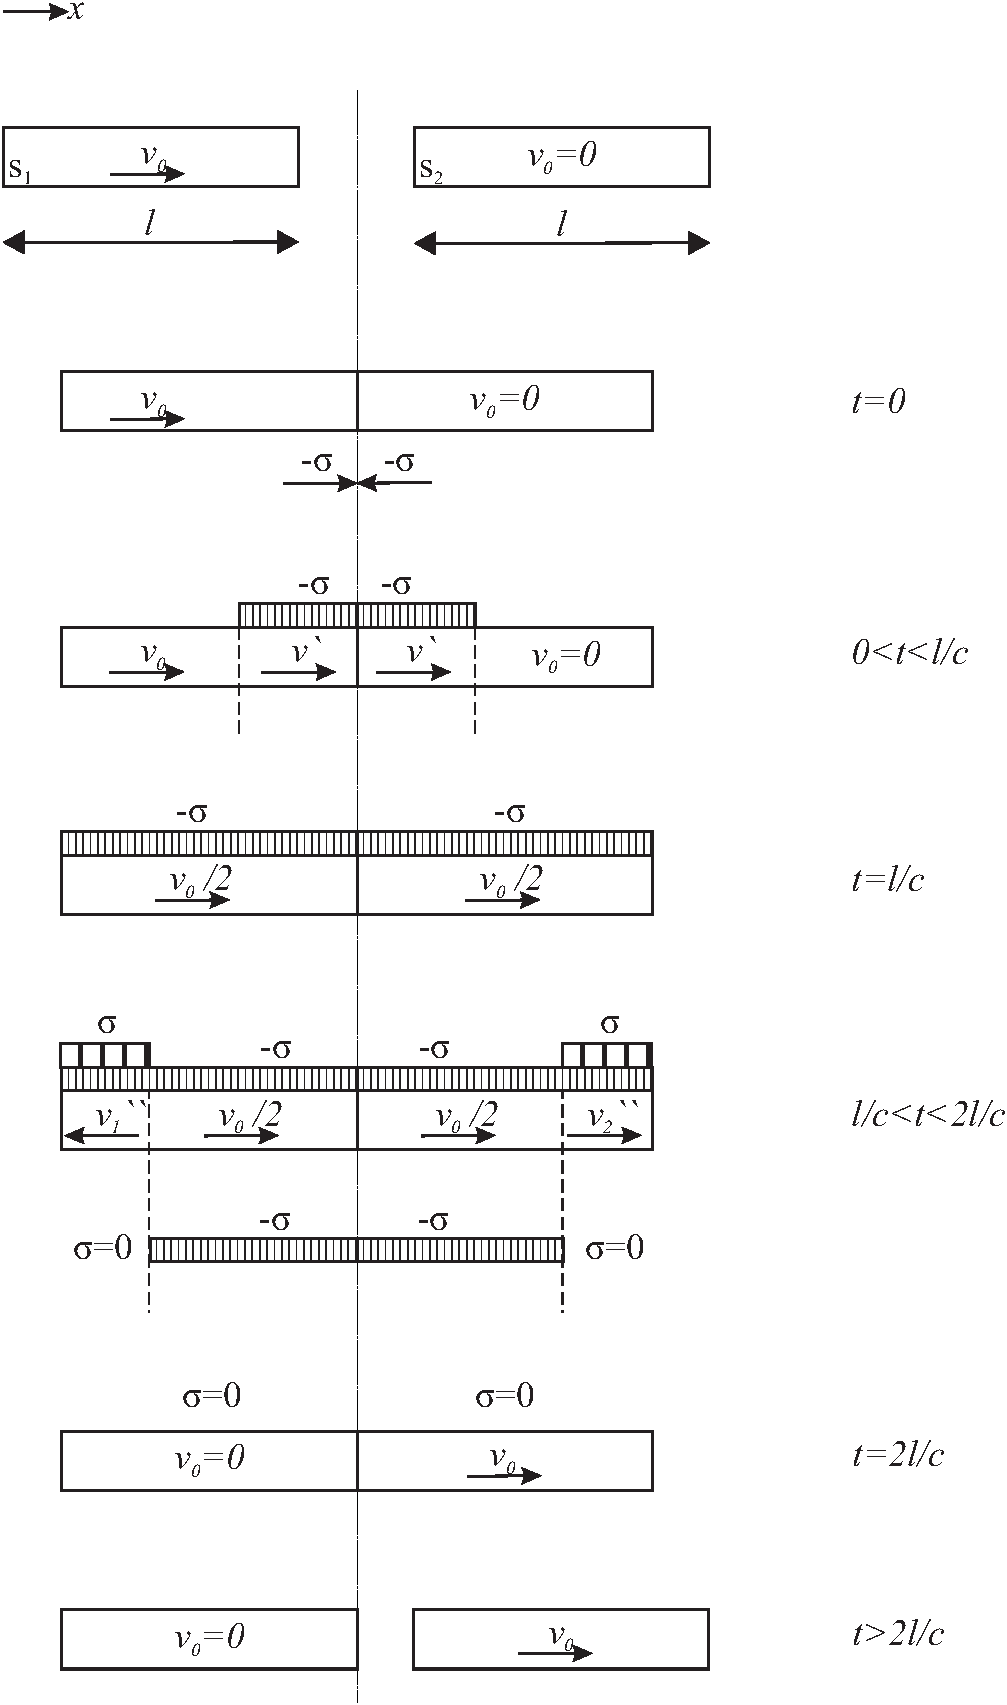
\includegraphics[width = 0.8\textwidth ]{figures/impact_of_two_bars_dalembert_solution.pdf}
    \caption{Different steps in the impact of two identical bars, one stationary and another with an initial velocity.}
    \label{fig:p2}
\end{figure}


% \newpage
% \bibliography{ref}
% \bibliographystyle{ieeetr}

\end{document}